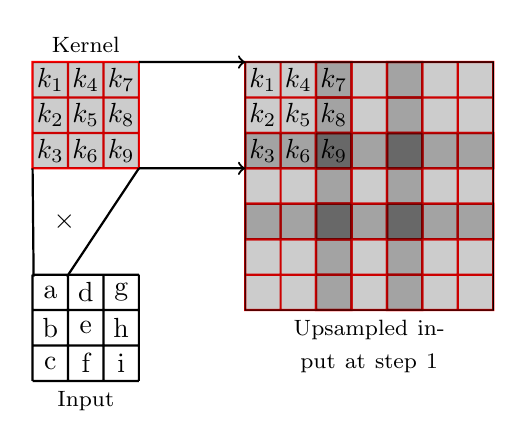
\begin{tikzpicture}
\begin{scope}[transparency group]
\begin{scope}[blend mode=multiply]
%stride 1
%kernel
\draw [thick, draw=red, fill=black!20!white,scale = .45] (-1,5) rectangle (2,8) grid (-1,5);
%kernel label
\draw [scale=.45,above] node at (0.5,8)  {\footnotesize Kernel};
%kernel components
\draw [scale=.45] node at (-0.5,7.5) {$k_1$};
\draw [scale=.45] node at (-0.5,6.5) {$k_2$};
\draw [scale=.45] node at (-0.5,5.5) {$k_3$};
\draw [scale=.45] node at (0.5,7.5)  {$k_4$};
\draw [scale=.45] node at (0.5,6.5)  {$k_5$};
\draw [scale=.45] node at (0.5,5.5)  {$k_6$};
\draw [scale=.45] node at (1.5,7.5)  {$k_7$};
\draw [scale=.45] node at (1.5,6.5)  {$k_8$};
\draw [scale=.45] node (k9) at (1.5,5.5)  {$k_9$};
%kernel on output
\draw [scale=.45] node at (5.5,7.5) {$k_1$};
\draw [scale=.45] node at (5.5,6.5) {$k_2$};
\draw [scale=.45] node at (5.5,5.5) {$k_3$};
\draw [scale=.45] node at (6.5,7.5)  {$k_4$};
\draw [scale=.45] node at (6.5,6.5)  {$k_5$};
\draw [scale=.45] node at (6.5,5.5)  {$k_6$};
\draw [scale=.45] node at (7.5,7.5)  {$k_7$};
\draw [scale=.45] node at (7.5,6.5)  {$k_8$};
\draw [scale=.45] node at (7.5,5.5)  {$k_9$};
%Kernel label
\draw [thick, draw=black,scale=.45] (-1,-1) grid  (2,2) node at (0.5,-1)[below] {\footnotesize Input};
% step 1 featuremap
\draw [thin, draw=black ,scale = .45] (5,1) rectangle  (12,8) node at (8.5,1) [below,text width=3cm,align= center] {\footnotesize Upsampled input at step 1};
%draw abc step 1
\draw [scale=.45] node (a) at (-.5,1.5) {a};
\draw [scale=.45] node at (-.5,0.5) {b};
\draw [scale=.45] node at (-.5,-.5) {c};
\draw [scale=.45] node at (0.5,1.5) {d};
\draw [scale=.45] node at (0.5,0.5) {e};
\draw [scale=.45] node at (0.5,-.5) {f};
\draw [scale=.45] node at (1.5,1.5) {g};
\draw [scale=.45] node at (1.5,0.5) {h};
\draw [scale=.45] node at (1.5,-.5) {i};
%draw connections
\draw [thick,scale=.45] (a.north east) -- (2,5) {};
\draw [thick,scale=.45] (a.north west) -- (-1,5){};
\draw [->,thick,scale=.45] (2,5) -- (5,5){};
\draw [->,thick,scale=.45] (2,8) -- (5,8){};
\draw [scale=.45,thick] node at (-.1,3.5) {$\mathbf{\times}$};
%draw kernel positions 
\foreach \i in {1,3,5}
\foreach \j in {5,7,9}
	\draw [thick, draw=red, fill=black!20!white,scale = .45] (\j,\i) grid  (\j+3,\i+3) rectangle (\j,\i);
\end{scope}
\end{scope}
\end{tikzpicture}
